\chapter{Realisierung}\label{ch:realisierung}
In diesem Kapitel wird beschrieben, wie die Aufgabe dieser Arbeit gelöst wurde.
Dazu wird nach der im Kapitel \ref{ch:vorgehensweise} beschriebenen Reihenfolge der Arbeitsschritte vorgegangen.
Es ist nochmal zu erwähnen, dass zunächst die Provisionierung einer CICS-Instanz untersucht wird.
Danach wird in weiteren Schritten zuerst eine Db2 Datenbank und schließlich IBM MQ Queues dem Bereitstellungsprozess hinzugefügt.
Die Funktionsfähigkeit der so generierten Laufzeitumgebung wird mittels eines Testablaufes am Beispiel der DATEV-Rechnungsschreibung  sichergestellt. 
Es folgt eine Bewertung der implementierten Provisionierungslösung durch die Stakeholder bei DATEV e.G. (Entwickler, Administration, Technologiestrategie).
Zuletzt wird noch ein Fazit zur Realisierung gezogen und ein Ausblick im Bezug auf die technischen Aspekte gegeben.

\section{Testplex}
Vor Beginn der eigentlichen Untersuchung mussten zunächst alle benötigten Rechte beantragt werden.
Hierzu zählen unter anderem die Rechte für die Nutzung des Test-Plexes, die Nutzung von z/OSMF und z/OSPT und die Rechte für die Templateverwaltung innerhalb von z/OSMF.
Außerdem war es auf dem Testplex möglich, die Rechte für das Erstellen der CICS Dateien, das Recht, um eine CICS-Instanz starten zu dürfen und die Rechte für die Administration von Db2 und IBM MQ einer persönlichen UserID zu geben.
Dies stellt kein Problem dar, weil es sich bei dem Testplex um eine reine Systemtestumgebung handelt.
Das \glqq IBM Cloud and Management for z/OS\grqq-Toolkit benötigt lesenden Zugriff auf den Speicherpfad der Template Dateien.
Schließlich konnte mit dem ersten Versuch, ein bei der Installation von z/OSMF mitgeliefertes minimales CICS Template zu provisionieren, begonnen werden.

\subsection{IBM Standard CICS Template}
Trotz der Vorteile durch die Weboberfläche von z/OSMF wurde zunächst auf z/OSPT gesetzt.
Diese Entscheidung fiel auf Grund der höheren Flexibilität von z/OSPT, durch das Konzept der Images\footnote{Beschreibung siehe Absatz \ref{sssec:zospt}}.
Da es sich um ein mitgeliefertes Template handelt, sind alle benötigten Workflow Definitionsdateien und Template Dateien vorhanden.
Somit konnte mittels des Konsolenbefehesl \glqq zospt build\grqq{} ein Image erzeugt werden.
Jedoch zeigte sich ein weiterer Nachteil des Kommandozeileninterfaces, es ist nicht möglich Templates eine Domain und einen Tenant zuzuweisen.
Dies hatte zur Folge, dass der Befehl \glqq zospt build\grqq{} fehlschlug.
Für alle folgenden Aufgaben wurde deshalb z/OSMF genutzt.

Um das Template in die Software Services\footnote{Beschreibung in Absatz \ref{sssec:zosmf}} von z/OSMF aufzunehmen, sind die Template- und Workflow-Dateien in einem Unix Dateisystem auf dem Großrechner abgelegt.
Dabei wurden ihm eine Domain und ein Tenant zugewiesen.
Bevor das Template provisioniert werden kann, müssen Änderungen in der Variableinputfile vorgenommen werden.
Dazu mussten die Werte, der in der Tabelle \ref{tab:cgsvars} genannten Variablen angepasst werden.
Die Kurzbeschreibungen und die Beschreibungen aller Variablen, die im Standard Template vorhanden sind, ist in \cite{IBM.2019} zu finden.
\begin{table}[h]
\centering
\begin{tabularx}{\textwidth}{X|X}
Variablenname & Kurzbeschreibung \\
\hline
DFH\_REGION\_SEC & Legt fest, ob für das CICS Sicherheit im Allgemeinen aktiviert ist. \\
\hline
DFH\_REGION\_SECPRFX & Wenn DFH\_REGION\_SEC gesetzt ist, legt den Namen Prefix bei Authentificationanfragen für Ressourcen fest. \\
\hline
DFH\_REGION\_APPLID & Applikations ID der zu provisionierenden CICS-Instance. \\
\hline
DFH\_LE\_HLQ & High-level qualifier\footnote{Erste Zeichen eines Dateinamens, wird zum Filtern genutzt} für die Sprachumgebung\footnote{Grundeinstellungen der Programmiersprachen COBOL, PLI und C. Mitgelieferte IBM Grundmodule} \\
\hline
DFH\_REGION\_HLQ & High-level qualifier für die CICS Dateien.\\
\hline
DFH\_REGION\_LOGSTREAM & Legt fest, wie die Log Dateien für die provisionierte CICS-Instanz erstellt werden sollen. \\
\hline
DFH\_STC\_ID & User ID mit dem die CICS-Instanz startet. \\
\hline
DFH\_REGION\_DFLTUSER & Default User ID für die CICS-Instanz. \\
\hline
DFH\_REGION\_VTAMNODE & Name des VTAM Knotens, wenn die CICS-Instanz hochfährt. \\
\hline
DFH\_REGION\_MEMLIMIT & Dem CICS maximal zur Verfügung stehender Speicherplatz. \\
\hline
DFH\_ZOS\_PROCLIB & Datei auf dem Großrechner, die den Job enthält, der für das Erzeugen der CICS-Instanz zuständig ist. \\
\hline
DFH\_ZOS\_VSAM\_VOLUME & Speichersystem auf welchem die Dateien gespeichert werden sollen. Entscheidung kann auch an das System abgeben werden. \\
\hline
DFH\_CICS\_USSHOME & Homeverzeichnes des Unix System Services \\
\hline
DFH\_CICS\_HLQ & High-level qualifier von dem CICS Installationsort. \\
\end{tabularx}
\caption{Zu verändernde Variablen im minimalen CICS Template}
\label{tab:cgsvars}
\end{table}
Mit Hilfe der z/OSMF Oberfläche konnte das Template akutalisiert und somit die Änderungen übernommen werden.

Als nächster Schritt wurde ein Testlauf und somit ein erster Versuch das Template zu provisionieren durchgeführt.
Dabei kam es anfangs zu Rechteproblemen, da die Anforderungen und Rahmenbedingungen der DATEV e.G. in dem standardisierten IBM Template natürlich nicht berücksichtigt waren, beispielsweise ist die Berechtigung für das Starten von Jobs von DATEV Vorgaben abhängig und CICS-Start-Mechanismen haben spezifische Anforderungen an die Eingabeparameter.
Nach den notwendigen Anpassungen funktionierte das Provisonieren und die definierten Aktionen des IBM Standard CICS Templates im DATEV Umfeld.

\subsubsection{DATEV e.G. spezifischen CICS Template}\label{sssec:datevcics}
Nachdem das minimale IBM Standard CICS Template funktionsfähig war und erste Erfahrungen mit z/OSMF gesammelt worden waren, wurde ein allgemeines, mitgeliefertes Template untersucht.
Ziel dieses nächsten Schritts war die Provisionierung einer funktionsfähigen DATEV e.G. spezifische CICS-Instanz.
Um dieses Template an die DATEV Umgebung anzupassen und letztendlich eine \glqq DATEV CICS-Instanz \grqq{} zu provisionieren, wurden folgende Schritte durchgeführt.

\begin{samepage}
\begin{itemize}
\item Analyse des bestehenden Templates und der darauffolgenden Minimalisierung
\item Umgang und Anpassung der CSD Datei
\item Anpassung der Jobs und Skripte mit Schwerpunkt auf der \glqq createCICS.jcl\grqq-Datei.
\end{itemize}
\end{samepage}

Die Analyse ergab, dass das mitgelieferte Template mit insgesamt 76 verwendeten Dateien sehr umfangreich ist.
Es zählen alle Dateien, die direkt mit dem Template in Verbindung stehen.
Im Zentrum des Templates steht die Workflow Definitionsdatei \glqq provision.xml \grqq{} mit circa 583 Zeilen Code.
In dieser sind alle Steps, die bei einer Provisionierung durchgeführt werden, definiert.
Das Template beinhaltet nicht nur die Möglichkeit, CICS-Instanzen mit unterschiedlichen Konfigurationen zu provisionieren, sondern auch, ob dies mit Skripten oder mit der REST-Api geschieht.
Zu diesen unterschiedliche Konfigurationen zählt unter anderem die Unterscheidung, ob die CICS-Instanz einem Sysplex hinzugefügt werden soll oder nicht.
Die Übersichtlichkeit des allgeminen Templates ist dadurch geringer.
So wurden neben allen für ein DATEV e.G. spezifischen CICS nicht notwendigen Dateien auch nicht benötigte Variablen und Steps entfernt.
Wie in der Tabelle \ref{tab:vglTemps} zu sehen ist, konnten dadurch circa die Hälfte der Dateien gelöscht werden und bei der provision.xml wurde ein Drittel an Quellcode eingespart werden.
Diese Version dient dem weiteren Vorgehen als Grundlage.

\begin{table}[h]
\centering
\begin{tabularx}{\textwidth}{r|X|X}
& IBM Standard CICS Template & DATEV e.G. spezifisches Template \\
\hline
Verwendete Dateien & 76 & 36 \\
\hline
provision.xml & circa 583 Codezeilen & circa 199 Codezeilen. \\
\end{tabularx}
\caption{Verlgeich des beiden Templates im Bezug auf deren Umfang}
\label{tab:vglTemps}
\end{table}

Als nächster Schritt wurde in Zusammenarbeit mit den CICS Administratorenteam festgelegt, wie im Umfeld der automatisierten Bereitstellung die CSD Dateien verwaltet werden soll.
Es wurde festgelegt, dass jede provisionierte CICS-Instanz ihre eigene CSD Datei zur Verfügung gestellt bekommen soll.
Hierfür soll die bestehende, von den Kollegen gepflegte Datei kopiert und mit bestimmten Namenkonventionen gespeichert werden.
Somit ist sichergestellt, dass durch die neu provisionierten Instanzen die existierenden und bei DATEV im Einsatz befindlichen Instanzen nicht beeinflusst werden.
Das ermöglicht auch jedem Nutzer der Provisionierung, die CSD seiner eigenen CICS-Instanz ohne Seiteneffekte zu bearbeiten.
Ein weiterer Vorteil ist, dass bei der Deprovisionierung der CICS-Instanz diese Kopie der Standard Datei ohne Nebenwirkungen gelöscht werden kann.
Dadurch, dass die Datei, die von den Kollegen gepflegt wird, als Grundlage verwendet wird, sind alle provisionierten Instanzen immer auf dem aktuellsten Stand.
Um dies umzusetzen, musste ein JCL Job geschrieben werden, der den Kopiervorgang implementiert.
Dieser Job wurde mittels eines neuen Steps in den z/OSMF Workflow eingebunden.
Außerdem mussten bestimmte Gruppen zu der CSD Liste der CICS-Instanz hinzugefügt werden.
Die JCL ist in Abbildung \ref{code:addCSD} dargestellt.
Die Reihenfolge ist relevant, da es der Initialisierungsreihenfolge entspricht.

\begin{minipage}{\linewidth}
\lstinputlisting[caption={Hinzufügen weiterer CSD Gruppen zur Liste der provisionierten CICS-Instanz mittels eines Jobs},captionpos=b,label={code:addCSD}]{listings/initaddCSDalt.jcl}
\end{minipage}

Im nächsten Schritt wurden die Jobs und Skripte angepasst.
Zunächst wurden die Namen der CICS Dateien\footnote{Beschreibung in Absatz \ref{sssec:speziDat}} an die DATEV e.G. internen Namenskonventionen angepasst.
Ein spezielles Augenmerk lag auf der Anpassung der \glqq createCICS.jcl\grqq-Datei.
In dieser befindet sich die Definition des STC Jobs für das provisionierte CICS.
Im Standard IBM Template beinhaltet diese zunächst ein Makro für die Validierung der SIT Parameter.
Zusätzlich werden noch bevor die Jobdefinition beginnt alle aus der Datei für die Eingabevariablen benötigten Variablenwerte in temporäre Zwischenvariablen eingefügt.
Danach folgt die Definition des Jobs, diese setzt sich aus folgenden Hauptbestandteilen zusammen:

\begin{samepage}
\begin{itemize}
\item Einbindung der benötigten Bibliotheken
\item Einbindung der zuvor angelegten CICS spezifischen Dateien
\item Definition der SIT Parameter
\end{itemize}
\end{samepage}

Sowohl bei die Einbindung der benötigten Bibliotheken als auch das Einbinden der zuvor angelegten CICS spezifischen Dateien beschränkte sich auf das Hinzufügen weiterer DD-Statements.

In Abbildung \ref{code:sitparams} ist zu sehen, dass es vor allem bei der Definition der SIT Parameter zu tief verschachtelten if-Bedingungen kommen kann.
Es handelt sich um den Code, der für das Einlesen der Variable \glqq DFH\_REGION\_SITPARAMS\grqq{} aus der Eingabedatei zuständig ist.
In dieser Variable werden die SIT Parameter als Komma separierter String angegeben.
Für die Erzeugung eines DATEV e.G. spezifischen CICS wurde das Makro für die Validierung von SIT Parametern beibehalten.
Alles danach wurde zunächst durch eine zur Verfügung gestellten DATEV e.G. Standard JCL, für die Erzeugung eines CICS, ersetzt.
Nach und nach wurde damit die notwendige Logik, wie die aus Abbildung \ref{gleiche abbildung wie oben}, hinzugefügt .
Damit wurde die vorher statische DATEV e.G. Standard JCL durch Verwendung von Template internen Variablen flexibilisiert.

\begin{minipage}{\linewidth}
\lstinputlisting[caption={Setzen der SIT Parameter durch Auslesen der \glqq DFH\_REGION\_SITPARAMS\grqq{} Variablen},captionpos=b,label={code:sitparams}]{listings/sitparams.jcl}
\end{minipage}

Es wurden nur die wirklich benötigten SIT Parameter aufgenommen.
Die anzunehmenden Werte wurden einzeln mit dem CICS Administratorenteam besprochen und festgelegt.
Es ist zu beachten, dass es im IBM Standard Template zwei Möglichkeiten gibt, diese Parameter zu setzen.
Für bestimmte SIT Parameter besteht eine Variable innerhalb des Templates.
Für alle anderen ist die Variable \glqq DFH\_REGION\_SITPARAMS\grqq{} vorgesehen.
In dieser Arbeit wurde hauptsächlich mit letzterer Variante gearbeitet.
Dadurch sind die SIT Parameter nur an einer Stelle im Template zu verwalten, beziehungsweise wird die Verwaltung  nicht auf zwei Arbeitsweisen verteilt.

Durch die beschriebene Vorgehensweie wurde erfolgreich die Provisionierung eines DATEV e.G. spezifischen CICS-Instanz umgesetzt.
Sichergestellt wurde dies mit einem Anmeldevorgang an dieses CICS, wie in Abbildung \ref{fig:cicslogin} zu sehen ist.
Außerdem sind alle Standard DATEV eG Transaktionen in dieser Instanz funktionsfähig.
Die Deprovisionierung verlief nach Plan.

\begin{figure}[h]
	\centering
	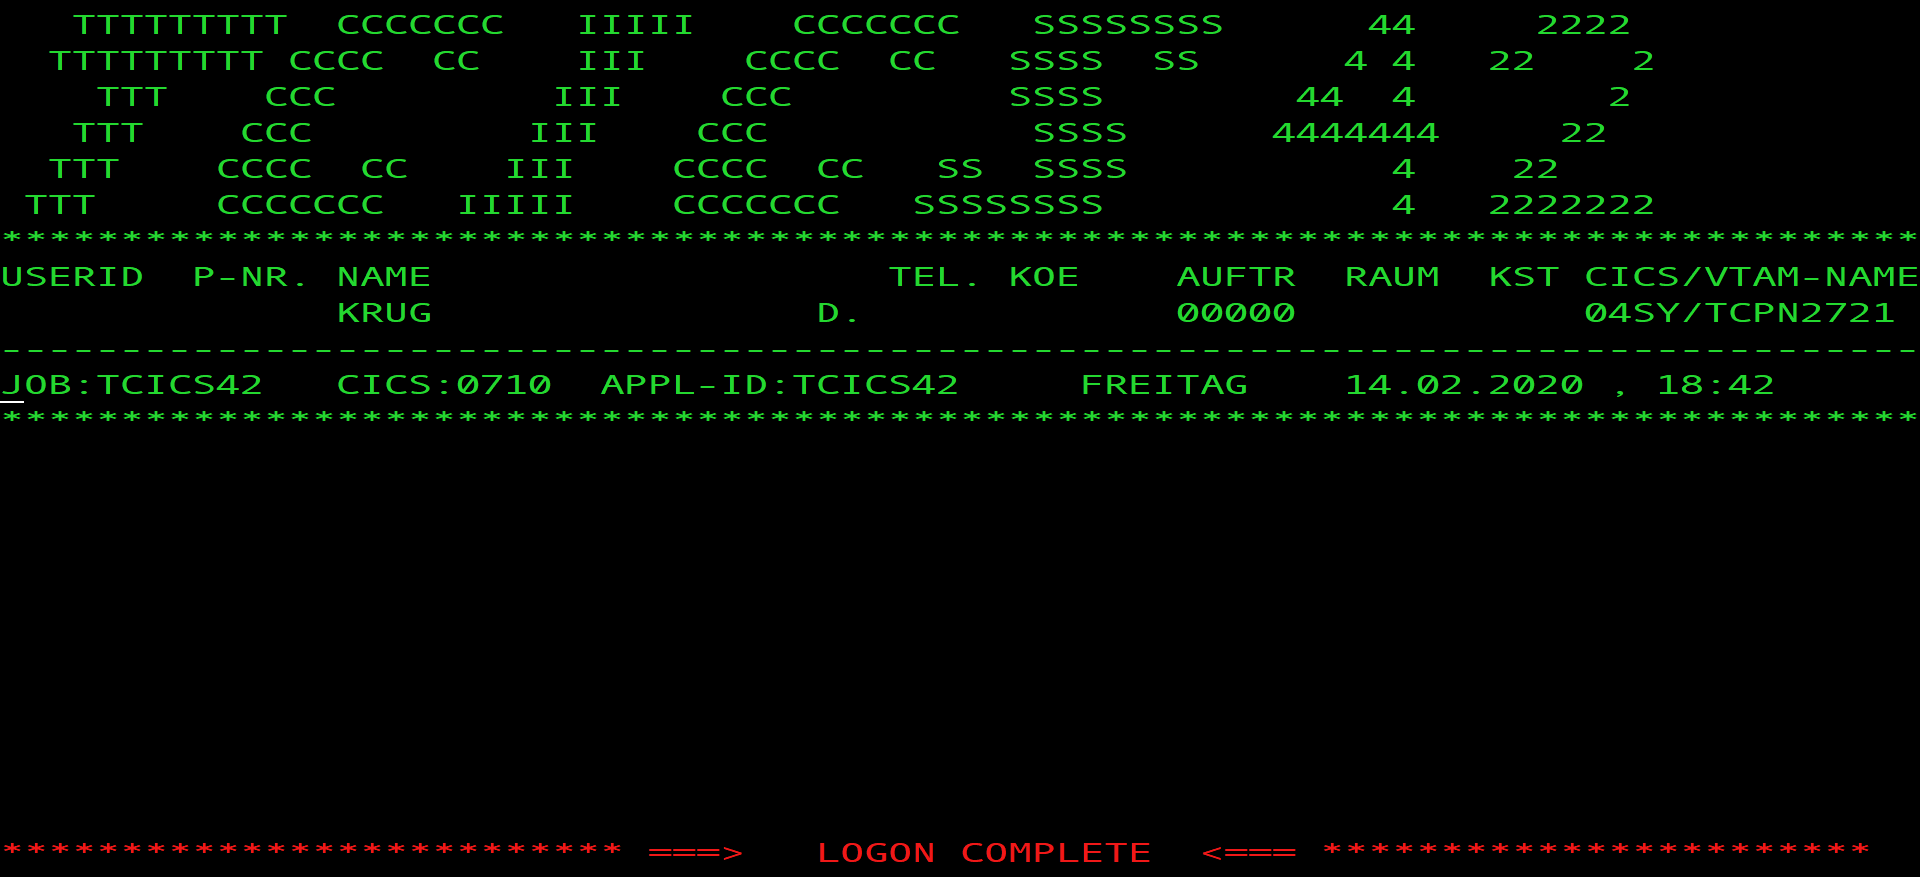
\includegraphics[width=\textwidth]{figures/logonscreen.PNG}
	\caption{Login Bildschirm der provisionierten DATEV spezifischen CICS-Instanz}
	\label{fig:cicslogin}
\end{figure}

\subsubsection{Bereitstellung Db2}\label{sssec:db2tpl}
In diesem Absatz wird die Provisionierung einer Db2 Datenbank beschrieben.
In der Systemumgebung Testplex bedeutet dies die Provisionierung der Datenbank ohne Tabelle und Daten.

Für die Erstellung einer Db2 Datenbank existiert innerhalb der DATEV e.G. eine REST-API.
Wie im Absatz \ref{sssec:workflow} beschrieben, ist es möglich, innerhalb eines Workflow Steps einen REST-Request abzusenden.
Der Code ist in Abbildung \ref{app:db2prov} im Anhang zu finden.
So muss im Body des Requests unter anderem der Datenbankname und eine UserID übergeben werden.
Der Code für das Löschen der Datenbank sieht ähnlich aus, nur handelt es sich in diesem Fall um einen DELETE-Request.
Die zwei notwendigen Steps wurden erzeugt und in den Workflow eingebunden.

Die API ist nur dazu fähig, Datenbanken auf einem bestimmten Datenbanksystem zu erzeugen.
Um die Datenbank aus der CICS-Instanz heraus nutzen zu können, muss dem CICS dieses Datenbanksystem mitgeteilt werden.
Hierfür ist, wie in Abbildung \ref{code:addCSD} in Zeile acht bereits zu sehen ist, das Hinzufügen einer weiteren CSD Gruppe notwendig ist, sowie die Aufnahme weitere Bibliotheken in der \glqq createCICS.jcl\grqq.
Dieser Aufruf wurde mittels neuer Variablen im Template möglichst dynamisch gestaltet und mussten in der Variableinputfile gesetzt werden.

\subsubsection{Bereitstellung IBM MQ}\label{sssec:mqtplx}
In diesem Absatz wird die Provisionierung einer IBM MQ Queue im Testplex beschrieben. 
Es ist auch möglich einen IBM MQ Queue Manager zu provisionieren, der Fokus dieser Arbeit liegt aber auf der Bereitstellung von Queues. 
Für die Bereitstellung eines IBM MQ Queue Mangers bei DATEV e.G. ist laut IBM MQ-Administration vorerst keine automatische Bereitstellung vorgesehen, gegebenenfalls kann dies in einem zukünftigen Szenario umgesetzt werden.
Ebenfalls in Abstimmung mit MQ- und CICS-Administration wurde entschieden, die Funktion eines Starts einer CICS Transaktionen über eine Queue vorerst nicht umzusetzen. Der Fokus lag auf der Prüfung, wie es möglich ist, eine einzelne Queue zu provisionieren, nicht die voll umfängliche Umsetzung der Anforderung der Anwendung DATEV-Rechnungsschreibung. 

Die IBM stellt Programme für die Verwaltung und das Nutzen von Queues  zur Verfügung.
Diese können mittels eines Jobs und bestimmten Parametern gestartet werden.
In Abbildung \ref{code:defq} ist die JCL des Jobs für das Erstellen einer Queue zu sehen.
Das auszuführende Programm ist \glqq CSQUTIL\grqq{} und als Parameter wird der Queuemanager übergeben.
Unter dem DD Namen \glqq MQSCIN\grqq{} ist der IBM MQ Befehl für das Erzeugen einer Queue zu sehen.
Um zu Prüfen, ob die Queue auch funktionsfähig ist, wurde nach dem Erstellen auch mit Hilfe eines Jobs, eine Message auf die Queue geschrieben und wieder abgeholt.
Der Job für das Löschen der Queues ist analog aufgebaut.

\begin{figure}[h]
	\centering
	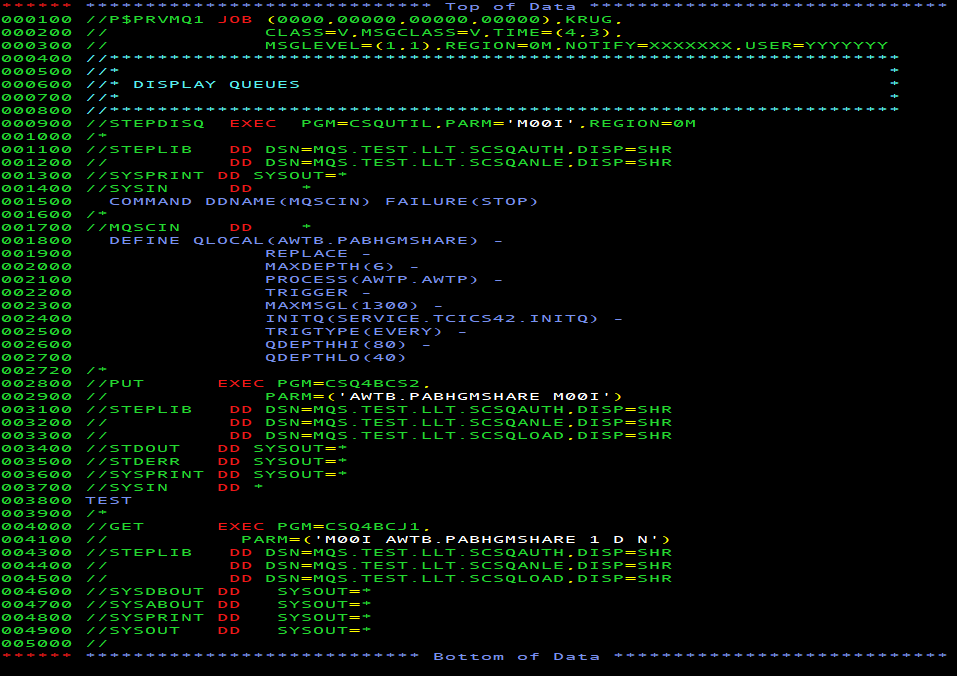
\includegraphics[width=\textwidth]{figures/defqjcl.PNG}
	\caption{Define IBM Queue, am Beispiel einer Trigger Queue}
	\label{code:defq}
\end{figure}

Ähnlich wie in Absatz \ref{sssec:db2tpl} für die Datenbank-Provisionierung beschrieben, muss der CSD Datei eine weitere Gruppe für den Queuemanager angegeben werden.
Zu sehen in Abbildung \ref{code:addCSD} in Zeile 11.
Dadurch hat die CICS-Instanz Zugriff auf alle Queues, die sich innerhalb dieses Managers befinden.
Des Weiteren ist die Aufnahme weiterer Bibliotheken in der \glqq createCICS.jcl\grqq{} notwendig.

\section{Entwicklungsstage}
Innerhalb der Entwicklungsstage sind die Sicherheits- und Rechtevorschriften schärfer als auf dem Test-Plex.
So wäre es zwar möglich, alle für die administrativen Aufgaben notwendigen Rechte einer persönlichen UserID zu geben.
Dies würde bedeuten, dass alle Anwender dieses Templates diese Rechte auch benötigen.
Damit bestünde eine potentielle Gefahr für das System, da sie damit auch außerhalb des Templates diese Rechte besitzen würden.
Somit wurde in Absprache mit den Administratorenteams für CICS und IBM MQ festgelegt, hierfür jeweils einen technischen User\footnote{User ID mit zunächst keinen Berechtigungen} zu beantragen.
Diesem werden nur die für das Template benötigten Rechte übergeben und er ist somit use-case-spezifisch.
Um als Anwender das Template nutzen zu können, werden nur die Rechte benötigt, Jobs mit diesen technischen Usern ausführen zu dürfen.
Für Db2 ist ein solcher User nicht notwendig, da das Datenbanksystem hinter der REST-API für alle zugänglich ist und jeder darauf Datenbanken erstellen darf.

Bei der Übertragung des Templates vom Test-Plex in die Entwicklungsstage waren Anpassungen in allen drei Bereichen des Templates notwendig.

\subsection{CICS Anpassung}
Dass der CICS spezifische technische User zum Einsatz kommt, musste der \glqq Job\grqq{} Baustein jeder JCL in jedem Step modifiziert werden.
Dafür bietet z/OSMF die Möglichkeit beim Zuweisen des \glqq Tenants\grqq{} eine Standard Jobkarte, die vor jeden Job des Templates eingefügt wird, zu hinterlegen.
Die CICS spezifischen Dateien können von der täglichen Datensicherung der Entwicklungsstage ausgeschlossen werden.
Da diese bei der Deprovisionierung gelöscht werden.
Um dies zu gewährleisten musste der Messageclass Parameter mit dem Wert  \glqq NONE\grqq{} angegeben werden.

Außerdem wird die CSD Datei, die als Vorlage gilt, durch die Standard Entwicklungsstage CSD Datei ersetzt.
In der Entwicklungsstage kommen im Vergleich zum Testplex andere Db2 und IBM MQ Bibliotheken zum Einsatz.
Dahingehend wurde die \glqq createCICS.jcl\grqq-Datei angepasst.
Zusätzlich musste ein SIT Parameter angepasst werden, so dass die Log Dateien funktionisfähig sind.
Eine weitere CSD Gruppe musste hinzugefügt werden.
Siehe Zeile 16 im Codeabschnitt \ref{code:createGrp}.
Diese sorgt dafür, dass die Bibliotheken, die die kompilierten Programme der kompletten Entwicklungsstage beinhalten, zur Verfügung stehen.
Außerdem kam noch eine neue Bibliothek hinzu.
Diese dient später als Ablageort der kompilierten Programme, die explizit nur in diese CICS-Instanz vorhanden sind.
Dies ist ein Standardvorgehen innerhalb der DATEV e.G. um neue Programmversionen zu testen.

\subsection{Db2 Anpassung}\label{ssec:db2entw}
Eine genauere technische Analyse der DATEV-Rechnungsschreibungsdatenbank kam zu dem  Ergebnis, dass es zwar möglich wäre diese Datenbank zu provisionieren, dies aber den zeitlichen Rahmen dieser Arbeit übersteigen würde.
Der Grund hierfür ist die Komplexität der benötigten Tabellen.
So wird auf drei Tabellen für die Ermittlung der Produktstammdaten lesend zugegriffen, auf neun weitere bei der Bestimmung der Preisabhängigkeiten.
Auf die Tabellen wird nicht direkt zugegriffen, sondern über Views\footnote{Alias eines Datenbankabfrage, auf die wie auf eine normale Tabelle zugegriffen werden kann}.
Bei den meisten werden innerhalb der View noch weitere Tabellen, teilweise aus anderen Datenbanken, gejoint.
Insgesamt besteht das System aus 14 Tabellen, die auf vier Datenbanken aufgeteilt sind, und 12 Views für den Zugriff auf diese Tabellen.

Die Db2 Administration muss dafür Vorarbeit leisten.
Mit dieser wurde begonnen, jedoch stellte sich heraus, dass die Komplexität (circa 600 Zeilen Code\footnote{Data Definition Language im Anhang \ref{app:ddl} zufinden} für einen kleinen Teil an Tabellen) der Anwendung DATEV Rechnungsschreibung im Rahmen dieser Arbeit als zu umfangreich angesehen wurde.
Sollte sich die Provisionierung generell als zielführend erweisen wird dieser Einmalaufwand erbracht werden.

Für die weitere Arbeit werden Datenbanken, die in einem anderen Datenbanksystem bereits vorhanden sind, genutzt.
Hierfür mussten die dafür vorgesehenen Variablen in der Eingabedatei des Templates angepasst werden.
Dadurch ändert sich die Gruppe in Zeile acht im Codeabschnitt \ref{code:addCSD} von \glqq DB0C \grqq{} auf \glqq DB0T \grqq.
Außerdem wurden sowohl in der Provisionierungs- als auch in der Deprovisionierungsdatei die Datenbanksteps auskommentiert und somit kommen diese nicht mehr zum Einsatz.

\subsection{IBM MQ Anpassung}\label{ssec:mqentw}
Da für die DATEV Rechnungsschreibung, wie im Absatz \ref{ssec:recharch} beschrieben, sehr viele gleichartige Queues benötigt werden, wurde für die Erstellung dieser von den IBM MQ Administratorenteam ein REXX Skript angefertigt.
Dies geschah unabhängig dieser Arbeit zum Zeitpunkt der Einführung des aktuellen DATEV Rechnungsschreibungsprozesses.
Dieses Skript steht dieser Arbeit zur Verfügung.
Für die Provisionierung IBM MQ Queues waren folgende Arbeitsschritte notwendig.

\begin{samepage}
\begin{itemize}
\item Anpassung des zur Verfügung stehenden Skriptes
\item Implementierung von Jobs für restliche Queues
\item Anpassung der CICS CSD Datei
\end{itemize}
\end{samepage}

Hierfür wurden zunächst die Eingabeparameter durch vorher angelegte Templatevariablen ersetzt.
Diese steuern, wie viele Queues jeweils angelegt werden, auf welchen Queue Manager die Queues angelegt werden und den ersten Qualifier des Queuenamens.
Für den restlichen Queuenamen existiert auch eine Variable, in dieser werden die Namen als Komma separierte Liste angeben und ausgelesen.
Anhand dieser Namen wird dann die maximale Queuetiefe und die maximale Länge einer einzelnen Nachricht festgelegt.
Im alten Skript wurden die Queues mit Hilfe einer Queue, die als Vorlage dient, angelegt.
Im Fall einer Provisionierung kann nicht davon ausgegangen werden, dass diese Vorlagen zur Verfügung stehen.
Deshalb wurden die benötigten Parameter explizit manuell angegeben.
Um die damit erstellten Queues zu testen, wurde eine Routine entwicklelt, die eine Nachricht auf die Queue schreibt und diese wieder abholt.
Anschließend wurde das Skript in den Provisionierungsworkflow mit Hilfe eines neuen Steps aufgenommen.

Für die Deprovisionierung der Queues besteht noch kein Skript.
Als Grundlage kann das vorher angepasste Provisionierungsskript dienen.
Hierfür musste der \glqq Define\grqq-Befehl für die Erstellung von Queues durch den \glqq Delete\grqq-Befehl ausgetauscht werden.
Die Logik für die Ermittlung der maximalen Queuetiefe und der maximalen Nachrichtenlänge wird dafür nicht mehr benötigt und konnte entfernt werden.

Die durch die beiden Skripte erstellten Queues sind nur für den Datenaustausch zwischen der CICS Transaktion für die Preisermittlung und dem Batch Ablauf zuständig.
Wie in Absatz \ref{ssec:recharch} beschrieben, benötigt der Ablauf noch weitere Queues.
Da es sich hierbei um spezielle Queues handelt, wurde auf die im Absatz \ref{sssec:mqtplx} gezeigte Technik zurückgegriffen.
Bei der Antwort-Queue für die Ermittlung der Listenpreise handelt es sich um eine Queue ohne besondere Parameter.
Es werden noch zwei Trigger-Queues benötigt, die über Prozesse eine Transaktion im CICS starten.
Als letzter Baustein für das Triggering der Transaktion wird noch eine Initiation Queue benötigt.
Diese muss im CICS hinterlegt sein.

Jeder CICS-Instanz kann nur eine Initiation Queue zugewiesen sein.
Dadurch benötigt jedes CICS eine eigene Initiation Queue.
Die Zuweisung geschieht in der IBM MQ CSD Gruppe.
Somit müsste für jede provisionierte CICS-Instanz im Voraus eine solche CSD Gruppe angelegt werden.
In Absprache mit der IBM MQ-Administrations  wurde entschieden, die Verwaltung der IBM MQ CSD Gruppe komplett dem Template zu übergeben.
Diese Entscheidung hatte eine Änderung des in Abbildung \ref{code:addCSD} gezeigten Codes zur Folge.
So wird, wie in Abbildung \ref{code:createGrp} dargestellt, zunächst eine Gruppe angelegt und erst anschließend dem CSD hinzugefügt.

\begin{minipage}{\linewidth}
\lstinputlisting[caption={Erstellung einer neuen CSD Gruppe},captionpos=b,label={code:createGrp}]{listings/InitAdditionalCSD.jcl}
\end{minipage}

Für jeden IBM MQ bezogenen Job wurde zuallerletzt die Jobkarte angepasst und der technische User der CICS-Administration durch den technischen User der IBM MQ-Admninistration, der für administrative Aufgaben berechtigt ist, ausgetauscht.

\subsection{Testablauf}
Für die Prüfung der Funktionsfähigkeit der so generierten Laufzeitumgebung steht dieser Arbeit ein Testablauf zur Verfügung.
Dieser wurde von den Mitarbeitern der DATEV Rechnungsschreibung beigesteuert.
Dabei handelt es sich um einen Teilablauf des gesamten DATEV Rechnungsschreibungsprozesses.
In diesem Ablauf wird nur die Preisermittlung, die die Laufzeitumgebung CICS benötigt, getestet.
Als Eingabe dienen vordefinierte Dateien und die Ergebnisse werden ebenfalls in Dateien geschrieben.
Der Ablauf liegt in Form von zwei Jobs vor.
Beide sind in der gleichen JCL Datei definiert, somit starten beide zeitgleich.
Dies ist notwendig, da der erste Job die Verarbeitung im CICS über die Queues startet und der zweite auf die Ergebnisqueues lauscht.

Um den Ablauf auch auf der vorher provisionierten Laufzeitumgebung zu starten, musste lediglich der verwendete Queue Manager angepasst werden.
Über die Queues und das verwendete Triggering wird die Transaktion im richtigen CICS gestartet.
Um die Ausgabe zu prüfen wurde der gleiche Testablauf mit den gleichen Eingabedateien auf der für Testzwecke üblichen Laufzeitumgebung durchgeführt.
Anschließend wurden die Ausgabedateien beider Läufe verglichen.

\section{Bereitstellungsprozess aktuelles Template}\label{sec:akttemp}
Bei dem Bereistellungsprozess, der durch das aktuelle Template möglich gemacht wird, sind drei Fälle zu unterscheiden:

\begin{samepage}
\begin{enumerate}
\item Fall:\\
Dem Entwicklerteam steht das Template in z/OSMF zur Verfügung und es wurde noch keine Instanz dieses Templates provisioniert.
Es wird eine neue Instanz benötigt.
\item Fall:\\
Dem Entwicklerteam steht das Template in z/OSMF zur Verfügung und es steht bereits eine Instanz dieses Templates zur Verfügung.
Es wird eine weitere Instanz benötigt.
\item Fall:\\
Das Administratorenteam führt Änderungen an einer Workflow Definitionsdatei durch.
Hier ist zwischen zwei weiteren Fällen zu unterscheiden:
\begin{enumerate}
\item Das Template wurde noch nicht veröffentlicht.
\item Das Template wurde veröffentlicht.
\end{enumerate}
\end{enumerate}
\end{samepage}

\subsection{1. Fall}
Der Mitarbeiter meldet sich an der zOSMF Oberfläche an und klickt auf den Menüleistenpunkt \glqq Cloud Provisioning\grqq.
Anschließend öffnet er die \glqq Software Services\grqq{} und wählt dort das oben genannte Template aus.
Er kann es ohne Änderungen provisionieren und damit seine Programmabläufe testen.

\subsection{2. Fall}\label{ssec:akttemp2fall}
Mit dem aktuellen Stand muss der Mitarbeiter wissen, an welchem Speicherort das Template abgelegt ist, da er die Template - nicht die Workflowdateien - kopieren muss.
Es sind Änderungen der Variableinputfile notwendig.
Unter anderem ist eine andere CICS Application ID zu wählen.
Um die Queues und IBM MQ Prozesse aus Fall eins nicht zu überschreiben, muss  ein anderer Queue Manager gesetzt werden.
Dieser Queue Manager muss von den zuständigen Administratorenteam manuell bereitgestellt werden.
Die Erzeugung einer von Fall eins unabhängigen Instanz setzt die Aufnahme eines neuen Templates, welches die veränderten Dateien beinhalten, in z/OSMF voraus.

\subsection{3. Fall}
Ein Template ist dann veröffentlicht, wenn es den berechtigten Teams zur Verfügung steht.
Zunächst muss der Speicherort der zu bearbeiteten Dateien bekannt sein.
Anschließend kann die Änderung mit einem Editor nach Wahl durchgeführt werden.

\subsubsection{3. Fall a)}
Hier kann das Template in der z/OSMF Oberfläche per Mausklick aktualisiert werden.

\subsubsection{3. Fall b)}
Um die Funktionsfähigkeit der veralteten Instanzen weiterhin sicherzustellen, muss eine neue Version des Templates erzeugt werden.
Dies ist auch per Mausklick zu lösen.

\section{Fazit Realisierung}
Am Ende der Realisierung steht ein funktionsfähiges Template.
Dieses Template provisioniert ein CICS und die benötigten IBM MQ Queues.
Wie in Absatz \ref{ssec:db2entw} beschrieben, wurde eine Db2 Datenbank wegen hoher Komplexität außen vorgelassen.
Auf dem Testplex wurde bewiesen, dass die Provisionierung einer Datenbank möglich ist.
Des Weiteren wäre die Provisionierung von Tabellen mit hohem einmaligen Arbeitsaufwand ebenfalls möglich.
Ein Testablauf der Beispielanwendung DATEV Rechnungsschreibung in einer provisionierten, isolierten CICS-Laufzeitumgebung konnte korrekt durchgeführt werden.

Folgende Probleme wurden im Rahmen der Implementierung erkannt:

\begin{samepage}
\begin{itemize}
\item Nicht sprechende Fehlermeldungen von z/OSMF
\item Nicht identifizierbare Programmiersprache
\item Nicht optimales Zugriffsrechtekonzept
\end{itemize}
\end{samepage}

Als erstes Problem sind nicht sprechenden Fehlermeldungen von z/OSMF, Abbildung \ref{fig:zosmffehler}, zu nennen.
\begin{figure}[h]
	\centering
	
\includegraphics[width=\textwidth]{figures/zosmffehlermeldung.png}
	\caption{Beispiel einer Fehlermeldung von zOSMF}
	\label{fig:zosmffehler}
\end{figure}
z.B. wird bei dem Hinzufügen und Aktualisieren eines Templates in z/OSMF das Template und damit alle davon benötigten Dateien auf Syntaxfehler geprüft.
Die in Abbildung \ref{fig:zosmffehler} gezeigte Meldung tritt dann ein, wenn ein solcher Syntaxfehler vorhanden ist.
Es ist aber nicht zu erkennen, welcher Fehler genau vorliegt, noch nicht einmal in welcher Datei dieser auftritt.
Zudem auch keine genaue Anzahl an auftretenden Fehlern.
Dieser Umstand, kombiniert mit 36 bestehenden Dateien, erschwert die Fehlersuche.
Im Gegensatz dazu wird im Fehlerfall beim Ausführen eines Steps immer der Fehlercode und der genaue Ort des Fehlers ausgegeben.
Beispielsweise wird bei einem Step, in dem ein REST Aufruf durchgeführt wird, und ein Fehler auftritt, der Requestcode und die hinterlegte Fehlermeldung an der z/OSMF Oberfläche angezeigt. 

Ein weiteres Problem ist eine nicht genau identifizierbare Programmiersprache, die für die dynamische Generierung von Skripten genutzt wird.
So ermöglicht diese die dynamische Wertzuweisung von zum Beispiel REXX-Variablen durch Variablen des Templates.
Außerdem besteht eine Art von String Verarbeitung.
Zu beachten ist, dass wenn am Zeilenanfang ein \glqq\#\grqq{} steht, kann diese Programmiersprache verwendet werden.
In Abbildung \ref{code:qsauslesen} ist ein Beispiel zu sehen.
Dort werden die Queuenamen, die als kommaseparierte Liste in der Templatevariable \glqq DFH\_MQ\_QUEUENAMES\grqq{} angegeben sind, ausgelesen und in eigenen REXX Variablen gespeichert.
Zu sehen ist zunächst eine \glqq set\grqq{} Anweisung, mit der Variablen zugewiesen werden können, If-Bedingungen und eine foreach-Schleife stehen außerdem zur Verfügung.

\begin{minipage}{\linewidth}
\lstinputlisting[caption={Auslesen der \glqq DFH\_MQ\_QUEUENAMES\grqq{} Variablen und schreiben in REXX Variablen},captionpos=b,label={code:qsauslesen}]{listings/qsauslesen.rexx}
\end{minipage}

In Abbildung \ref{code:qsauslesenlaufzeit} wird das Ergebnis, welches zur Laufzeit ausgeführt wird, dargestellt.
Es ist zu erkennen, dass nur noch die für das REXX Skript notwendigen Codeabschnitte vorhanden sind.
Dadurch können sehr dynamische Templates erstellt werden.
Jedoch wurde weder eine Dokumentation zu dieser Sprache, noch um welche Sprache es sich genau handelt gefunden.
Somit liegt dem Wissen über diese Sprache nur der Code aus Beispielen der IBM zu Grunde.

\begin{minipage}{\linewidth}
\lstinputlisting[language=Rexx,caption={Zur Laufzeit erzeugtes Skript, der Grundlage aus Codeabschnitt \ref{code:qsauslesen}},captionpos=b,label={code:qsauslesenlaufzeit}]{listings/qsauslesenlaufzeit.rexx}
\end{minipage}

Ein weiterer Problempunkt ist das mit z/OSMF und dem Template einhergehende Zugriffsrechtekonzept.
Die z/OSMF Berechtigungsgruppen sind nicht an die DATEV e.G. internen Richtlinien angepasst.
Die Aufnahme in eine solche Gruppe, um zum Beispiel die z/OSMF Oberfläche nutzen zu dürfen, geschieht auf Zuruf und manuelles Hinzufügen einer User ID durch einen Mitarbeiter.
Außerdem ist der Einsatz einer für das ganze Template gültigen Standard Jobkarte, um technische User verwenden zu können, nicht optimal.
z/OSMF bietet hier eigentlich eine Möglichkeit in der Stepdefinition einen \glqq runAsUser\grqq{} anzugeben.
Unter diesem User würde der Step dann ausgeführt werden.
Folglich ist das die Stelle an der zum Beispiel für CICS Steps der technische User für administrative CICS Aufgaben angegeben werden müsste.
So würde das Gewähren der expliziten Rechte zum Starten eines Jobs mit der technischen User Id entfallen und damit die manuelle Arbeit des \glqq Gewährens\grqq, was mittels eines Formulars beantragt wird.
Jedoch um einen \glqq runAsUser\grqq{} in der Stepdefinition angeben zu können, muss in der dem Template zugewiesen \glqq Domain\grqq{} ein sogenannter \glqq Cloud Security Admin\grqq{} hinterlegt sein.
Dieser würde sicherstellen, dass nur die für ein Template zugelassenen User dieses Template auch provisionieren dürfen.
In dieser Arbeit wird die mitgelieferte \glqq Default Domain\grqq{} genutzt, in dieser ist kein \glqq Cloud Security Admin\grqq{} angegeben.
Da es sich um die Standard \glqq Domain\grqq{} handelt, darf diese nicht geändert werden.
Somit müsste eine eigene \glqq Domain\grqq{} angelegt werden um einen \glqq Cloud Security Admin\grqq{} hinterlegen zu können.
Dadurch, dass sich z/OSMF bei der DATEV e.G. noch in einem Teststadium befindet, wird von der Erstellung einer eigenen \glqq Domain\grqq{} abgesehen.
Dies ist der Grund für den nicht optimalen Einsatz der oben genannten Jobkarten.
An diesen beiden Fällen ist zu erkennen, dass das Rechtekonzept noch nicht für einen firmenweiten Einsatz ausgelegt ist und noch überarbeitet und angepasst werden muss.
Dies ist jedoch explizit nicht Bestandteil dieser Arbeit.


 
